\documentclass[11pt,a4paper]{article}

\usepackage[T1]{fontenc}
\usepackage[utf8]{inputenc}
\usepackage{lmodern}
\usepackage[margin=2.3cm]{geometry}
\usepackage{amsmath,amssymb}
\usepackage{graphicx}
\usepackage{booktabs}
\usepackage{tabularx}
\usepackage{xcolor}
\usepackage{float}
\usepackage{caption}
\usepackage{enumitem}
\usepackage{parskip}
\usepackage{titlesec}
\usepackage{fancyhdr}
\usepackage{tcolorbox}
\usepackage{tikz}
\usetikzlibrary{arrows.meta,positioning,shapes.geometric,calc}
\usepackage[hidelinks]{hyperref}

\graphicspath{{figures/}{../paper/figures/}}
\definecolor{iimblue}{HTML}{1F4E79}
\definecolor{iimorange}{HTML}{C55A11}
\definecolor{boxgrey}{HTML}{F2F2F2}
\captionsetup{font=small,labelfont=bf,width=0.95\textwidth}
\setlist{nosep,leftmargin=1.5em,topsep=3pt}
\titleformat{\section}{\Large\bfseries\color{iimblue}}{\thesection}{0.8em}{}
\titleformat{\subsection}{\large\bfseries}{\thesubsection}{0.6em}{}
\pagestyle{fancy}
\fancyhf{}
\fancyhead[L]{\small Expiry days and the settlement price on NSE}
\fancyhead[R]{\small Project Course Report}
\fancyfoot[C]{\thepage}
\renewcommand{\headrulewidth}{0.4pt}
\setlength{\emergencystretch}{2em}

\newtcolorbox{takeaway}{colback=boxgrey,colframe=iimblue,boxrule=0.6pt,arc=2pt,
  left=6pt,right=6pt,top=4pt,bottom=4pt}
\newtcolorbox{whybox}{colback=white,colframe=iimorange,boxrule=0.6pt,arc=2pt,
  left=6pt,right=6pt,top=4pt,bottom=4pt,title={\small\bfseries Why does this happen?},
  coltitle=white,colbacktitle=iimorange}

\begin{document}

% ---------------------------------------------------------------- title page
\begin{titlepage}
\begin{tikzpicture}[remember picture,overlay]
  \draw[line width=0.6pt] ($(current page.north west)+(1.2cm,-1.2cm)$) rectangle
    ($(current page.south east)+(-1.2cm,1.2cm)$);
\end{tikzpicture}
\centering
\vspace*{0.6cm}

\includegraphics[width=4.6cm]{iima_logo.png}\par
\vspace{1.0cm}
{\LARGE\bfseries Project Course Report\par}
\vspace{0.7cm}
{\large\bfseries Term 5\par}
\vspace{1.1cm}
{\large\bfseries Academic Project\par}
{\large\itshape On\par}
\vspace{0.2cm}
{\Large\bfseries\color{iimblue} What Happens in the Last Half Hour?\par}
\vspace{0.2cm}
{\large\bfseries Expiry Days, the Settlement VWAP and the Order Book on the NSE\par}
\vspace{1.1cm}
{\large\bfseries Area\par}
{\large\bfseries FINANCE\par}
\vspace{1.1cm}
{\large\bfseries Name of the project supervisor:\par}
{\large Anirban Banerjee\par}
\vspace{1.1cm}
{\large\bfseries Name of the students:\par}
{\large Arnav Dixit (PGPGC202500112)\par}
{\large Mayank Gomekar (PGPGC202500150)\par}
\vfill
{\large November 2026\par}
\vspace*{0.4cm}
\end{titlepage}

\tableofcontents
\newpage

% ---------------------------------------------------------------- summary
\section{Summary}

Stock and index derivatives on the NSE settle at the volume-weighted average price (VWAP) of
the cash market between 15:00 and 15:30 on expiry day. Because so much money depends on these
thirty minutes, people often say that the settlement price gets ``punched'': traders with large
expiring positions push it one way. We wanted to check whether this happens and, if the window
does behave differently on expiry days, to understand why.

We used the NSE's complete order and trade files for 2022. For 24 sessions (the 12 monthly
expiries and the trading day before each) we rebuilt the full limit order book of 150 stocks
from about 10.9 billion order records. For all 242 sessions of the year we worked with the
trades, and for the expiry sessions we also rebuilt the order books of the expiring stock
futures. The 150 stocks are 50 heavily traded F\&O stocks, 50 less traded F\&O stocks, and 50
``placebo'' stocks that have no derivatives at all. Anything that also happens to the placebo
stocks on expiry day cannot be caused by the settlement.

\begin{figure}[H]
  \centering
  \includegraphics[width=\textwidth]{primary_tests.pdf}
  \caption{Our four main tests: the settlement window on expiry day against the same window on
    the day before, same stock, same month. Two of the four show a clear change.}
  \label{fig:primary}
\end{figure}

Our main findings, and the reasons we give for them:

\begin{enumerate}
  \item \textbf{Stock settlement prices are not pushed.} The settlement VWAP does not end up any
  further from where the window started (36.0 vs 34.5 bps, $p = 0.21$), and buying and selling in
  the window stay balanced. The reason is that stock F\&O are settled by physical delivery: a
  trader who holds a long future pays the agreed price for the shares whatever the settlement
  price turns out to be, so pushing it gains nothing. The futures price itself confirms this:
  near the close it follows the live cash price (slope 0.85), not the settlement VWAP.
  \item \textbf{The index is different, and it does fall.} The Nifty 50 is settled in cash, so
  here the settlement price really is the payoff. On the 52 index expiries of 2022 the Nifty 50
  falls 6.2 bps (about 11 index points) more than the Nifty Next 50, an index of similar stocks
  with no derivatives, over the window. A random-date test gives $p = 0.008$. Institutions sell
  Nifty 50 stocks in the window on these days, and they hold large index option hedges, which
  fits a story of hedges being closed at the settlement price. The size of the expiring
  positions, however, does not predict the size of the fall, so we cannot prove this story.
  \item \textbf{The window costs more to trade in on expiry day, only in F\&O stocks.} Spreads are
  about 10\% wider and the order book about 6\% thinner. The main reason is volatility: prices
  move about 45\% more in the window on expiry day in F\&O stocks (and barely more in placebo
  stocks), and market makers quote wider and smaller when prices move more. Volatility explains
  about 70\% of the wider spread and all of the thinner book.
  \item \textbf{More orders are cancelled within one second} (28.6\% to 30.1\%). This is also mostly
  volatility: market-making algorithms re-price every time the price moves.
  \item \textbf{The expiring stock future becomes very expensive to trade in the last half hour.}
  Its spread is 33\% wider on expiry day, three times the change in cash. Volatility explains only
  a third of this. Our explanation is that any futures position still open at 15:30 turns into a
  delivery of shares, so market makers step away from the expiring contract.
  \item \textbf{The partial fall in prices the next morning (Figure~\ref{fig:path}) is mostly
  news.} It is just as strong in placebo stocks, it comes from a handful of expiries, and it
  disappears once we adjust for overnight market moves and drop stock-days with signs of news.
\end{enumerate}

\begin{takeaway}
In one line: on expiry days the settlement window gets busier and more volatile, so it costs
more to trade in, but stock prices are not pushed because physical delivery removes the
incentive. The one settlement that does move is the cash-settled index.
\end{takeaway}

% ---------------------------------------------------------------- background
\section{Background: how settlement works on the NSE}

\subsection{The settlement price}

In 2022 equity derivatives on the NSE expired on the last Thursday of each month. The closing
price of a stock on that day is the final settlement price of its futures and the exercise
price used for its options. The closing price on the NSE is not the last trade of the day. It is
the VWAP of all trades between 15:00 and 15:30, the last half hour of continuous trading
(Figure~\ref{fig:timeline}).

\begin{figure}[H]
\centering
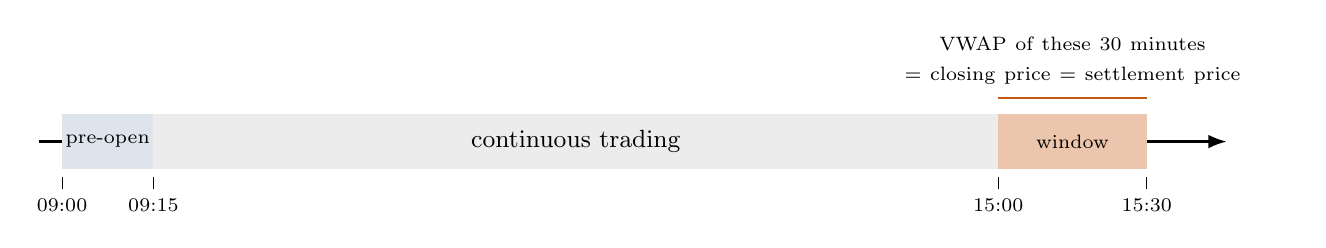
\begin{tikzpicture}[x=1.45cm,y=1cm,font=\small]
  \draw[thick,-{Latex}] (0,0) -- (10.4,0);
  \fill[iimblue!15] (0.2,-0.35) rectangle (1.0,0.35);
  \fill[gray!15] (1.0,-0.35) rectangle (8.4,0.35);
  \fill[iimorange!35] (8.4,-0.35) rectangle (9.7,0.35);
  \node at (0.6,0) {\scriptsize pre-open};
  \node at (4.7,0) {continuous trading};
  \node at (9.05,0) {\scriptsize window};
  \foreach \x/\t in {0.2/09:00,1.0/09:15,8.4/15:00,9.7/15:30} {
    \draw (\x,-0.45) -- (\x,-0.6); \node[below] at (\x,-0.6) {\scriptsize\t};}
  \draw[iimorange,thick] (8.4,0.55) -- (9.7,0.55);
  \node[above,align=center,text width=5.5cm] at (9.05,0.6) {\scriptsize VWAP of these 30 minutes\\
    = closing price = settlement price};
\end{tikzpicture}
\caption{A trading day on the NSE cash market. The settlement price of expiring derivatives is
  the VWAP of the shaded last half hour.}
\label{fig:timeline}
\end{figure}

Two types of settlement matter for this project:

\begin{itemize}
  \item \textbf{Stock futures and options are settled by delivery} (since 2019). A long future held
  to expiry becomes an obligation to take the shares, and an in-the-money option becomes a
  delivery at the strike. The settlement price decides the last margin payment on a future, but
  the trader still pays the original futures price for the shares in total.
  \item \textbf{Index futures and options (for example on the Nifty 50) are settled in cash}
  against the closing value of the index, which is calculated from the closing prices of its
  stocks. Index options also expired every Thursday in 2022 (weekly expiries), so most Thursdays
  carry an index settlement but no stock settlement.
\end{itemize}

\subsection{Why the window could be distorted}

The window is known in advance, it is short, and the settlement price is an average. A trader
who wants a higher or lower settlement price can plan trades through the window, and in a stock
that does not trade much, one trader's volume can be a big share of it. But moving an average is
costly: the trader pays the price impact on everything they trade, while the gain is only on
their expiring position.

There are also perfectly normal reasons for the window to look different on expiry day. Holders
of expiring positions who do not want delivery must close or roll them, and arbitrageurs who
hold shares against futures sell them at the settlement price, because that is the price at
which their futures settle. All of this adds volume to the window. So for every difference we
find, we ask whether it comes from someone pushing the price or simply from more people
trading.

% ---------------------------------------------------------------- hypotheses
\section{The four broad hypotheses}\label{sec:hyp}

Testing dozens of measures one by one would make the conclusion depend on how many of them
happen to be significant. So, as suggested, we grouped everything under four broad hypotheses
(BH), each with one primary measure decided in advance. The other measures are supporting
evidence. We control the false discovery rate across the four primary tests.

\begin{center}
\small
\begin{tabularx}{\textwidth}{lXXl}
\toprule
 & Hypothesis & Primary measure & Result \\
\midrule
BH1 & The settlement price behaves differently on expiry day &
  Distance of the settlement VWAP from the mid at 15:00 & Not rejected ($p=0.21$) \\
BH2 & Trading in the window costs more & Quoted spread & Rejected ($p<0.001$) \\
BH3 & Trading in the window is more one-sided & $|$OIB$|$ over the window & Not rejected ($p=0.54$) \\
BH4 & Order behaviour and participation change & Share of orders cancelled within 1 second &
  Rejected ($p<0.001$) \\
\bottomrule
\end{tabularx}
\end{center}

``Rejected'' here means we reject the null of no change, so BH2 and BH4 are supported. Each
measure is computed for each stock in the window, and the expiry day is compared with the
trading day before it in the same month.

% ---------------------------------------------------------------- data
\section{Data}

\subsection{What the NSE files contain}

The NSE sells complete order and trade files for every session. The \emph{order file} records
every order entry, modification and cancellation with a microsecond timestamp, buy or sell,
quantity (total and displayed), limit price, flags such as IOC, whether it came from an algorithm,
and the participant category: custodian (institutions such as FIIs and mutual funds),
proprietary (brokers trading their own money) or other clients. The \emph{trade file} records every
trade with the order numbers of the buyer and the seller. For the derivatives market the same
files exist with the contract, expiry, strike and option type.

\begin{center}
\small
\begin{tabularx}{\textwidth}{lXl}
\toprule
Sample & What it covers & Used for \\
\midrule
Order book sample & 24 sessions: 12 monthly expiries + day before each & spreads, depth, cancellations \\
 & 10.9 billion order records, 488 million trades & \\
Full-year trade sample & All 242 sessions of 2022, 36,300 stock-days & prices, flows, reversal \\
Index file & Nifty 50 and Nifty Next 50 every second, 243 sessions & index settlement \\
F\&O files & Trades and orders, all 12 expiries + day before & futures, index options \\
Public NSE files & Daily F\&O bhavcopy and participant-wise open interest & open interest, positions \\
\bottomrule
\end{tabularx}
\end{center}

The trade file for 2 August 2022 was corrupt, so the full-year sample has 242 of the 243 sessions.
One part of the derivatives order file for the April expiry was an incomplete download, which
costs us some futures for that one day.

\subsection{The three groups of stocks}

\begin{itemize}
  \item \textbf{Liquid F\&O}: the 50 most traded stocks that have stock derivatives (typical
  turnover about Rs 376 crore a day).
  \item \textbf{Illiquid F\&O}: the 50 least traded stocks with derivatives (about Rs 42 crore a day).
  Both F\&O groups face the same settlement incentive; for the illiquid ones, moving the price is
  cheaper.
  \item \textbf{Placebo}: 50 stocks with no derivatives at all, matched to the illiquid group on
  turnover and price (about Rs 38 crore a day). Nothing settles on their closing price, but they
  live through the same calendar.
\end{itemize}

We chose the groups using only the control days, so that expiry-day behaviour could not affect
which stocks were picked. Whether a stock has derivatives was read directly from the F\&O trade
files. No stock without derivatives trades as heavily as the liquid group, so the placebo
comparison really speaks to the illiquid group.

\subsection{Are the placebo stocks a fair comparison?}\label{sec:placebo}

Prof.\ Banerjee asked whether the placebo stocks are proper companies or a fringe of thinly traded
names. We checked them against the Nifty 500 list of October 2022 (an archived copy of NSE's
constituent file) and ranked every stock by turnover among the 1,129 equities traded on our
sessions.

\begin{figure}[H]
  \centering
  \includegraphics[width=\textwidth]{placebo_check.pdf}
  \caption{Left: turnover rank of each stock in our three groups. Right: how many were in the
    Nifty 500 in October 2022.}
  \label{fig:placebo}
\end{figure}

44 of the 50 placebo stocks were in the Nifty 500 in October 2022, and 48 were in it either in
July 2020 or in February 2024. Their median turnover rank is 244, close to the illiquid F\&O group
(219), and none of them had derivatives in 2022. They are established mid-cap companies, which is
exactly what a placebo for the illiquid F\&O group should be.

% ---------------------------------------------------------------- method
\section{Methodology}

\subsection{From raw files to measures}

\begin{figure}[H]
\centering
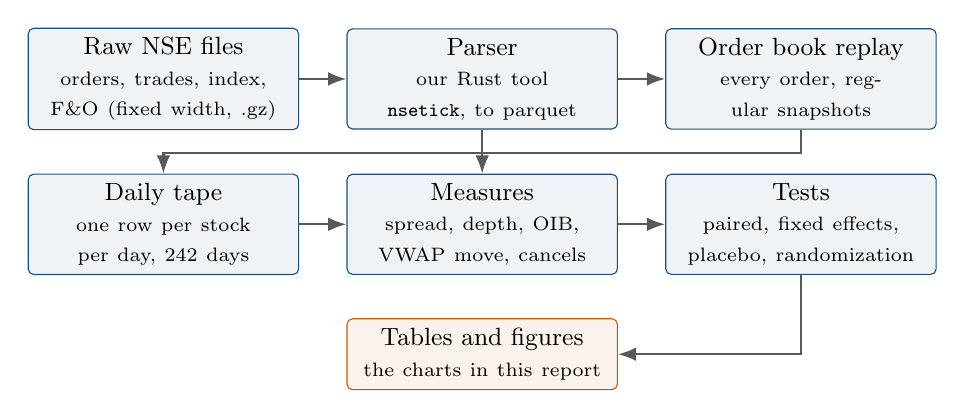
\begin{tikzpicture}[node distance=0.55cm and 0.6cm, font=\small,
  box/.style={draw=iimblue,fill=iimblue!7,rounded corners=2pt,align=center,
    minimum height=0.9cm,text width=3.2cm},
  outbox/.style={draw=iimorange,fill=iimorange!8,rounded corners=2pt,align=center,
    minimum height=0.9cm,text width=3.2cm},
  arr/.style={-{Latex},thick,color=gray!70!black}]
  \node[box] (raw) {Raw NSE files\\ \scriptsize orders, trades, index, F\&O (fixed width, .gz)};
  \node[box,right=of raw] (parse) {Parser\\ \scriptsize our Rust tool \texttt{nsetick}, to parquet};
  \node[box,right=of parse] (book) {Order book replay\\ \scriptsize every order, regular snapshots};
  \node[box,below=of raw] (tape) {Daily tape\\ \scriptsize one row per stock per day, 242 days};
  \node[box,right=of tape] (meas) {Measures\\ \scriptsize spread, depth, OIB, VWAP move, cancels};
  \node[box,right=of meas] (tests) {Tests\\ \scriptsize paired, fixed effects, placebo, randomization};
  \node[outbox,below=of meas] (rep) {Tables and figures\\ \scriptsize the charts in this report};
  \draw[arr] (raw) -- (parse); \draw[arr] (parse) -- (book);
  \draw[arr] (parse.south) -- ++(0,-0.3) -| (tape.north);
  \draw[arr] (book.south) -- ++(0,-0.3) -| (meas.north);
  \draw[arr] (tape) -- (meas); \draw[arr] (meas) -- (tests);
  \draw[arr] (tests.south) |- (rep.east);
\end{tikzpicture}
\caption{How we went from the exchange's files to results. The heavy steps ran on a high-performance computing server.}
\label{fig:pipeline}
\end{figure}

\paragraph{Parsing.} The NSE files are fixed-width text in a layout that changed during the year.
We wrote a parser (\texttt{nsetick}, in Rust) that decodes each file with the right layout, checks
the record length, and writes parquet files split by date and stock. Timestamps come as
``jiffies'' (units of 1/65536 of a second) and prices in paise.

\paragraph{Rebuilding the order book.} For each stock and session we replay every order event in
sequence: entries add to the book, modifications move orders, cancellations remove them, and
trades consume them. Orders with a disclosed quantity show only the displayed part, and the
hidden part refills as it trades, losing its place in the queue. We take a snapshot of the book
every few seconds (20 price levels per side) and read off the best bid and ask, depth, hidden
size, and how many orders arrived and were cancelled in between.

\paragraph{Who initiated a trade.} Order numbers are assigned in the order orders arrive. In every
trade, the order with the larger number arrived second and crossed the spread, so it is the
aggressor. This gives us the true direction of every trade, with no need for a classification
rule such as Lee and Ready's.

\subsection{Main measures}

\begin{center}
\small
\begin{tabularx}{\textwidth}{lX}
\toprule
Measure & How we compute it \\
\midrule
Settlement VWAP & VWAP of all regular trades from 15:00 to 15:30 \\
Window move & $10^4 \ln(\text{settlement VWAP} / \text{VWAP of 14:50 to 15:00})$, in bps \\
Next-morning return & $10^4 \ln(\text{VWAP of next day's first 30 min} / \text{settlement VWAP})$ \\
Quoted spread & $(\text{ask} - \text{bid})/\text{mid}$, averaged over the window, in bps \\
Depth & Rupee value of displayed orders within 5 price levels on each side \\
OIB & $(BI-SI)/(BI+SI)$, buyer- minus seller-initiated volume over total \\
Fleeting orders & Share of orders cancelled within one second of entry \\
Volatility & Sum of squared 5-second changes of the log mid price \\
Net aggressor flow & Aggressive buying minus aggressive selling, \% of the stock's median daily volume \\
\bottomrule
\end{tabularx}
\end{center}

\subsection{Statistical tests}

\begin{itemize}
  \item \textbf{Paired comparison.} For each stock, the expiry day minus the day before in the same
  month (about 1,800 stock-month pairs). This removes anything specific to the stock or the month.
  \item \textbf{Placebo comparison (difference in differences).} Is the expiry-day change in F\&O
  stocks bigger than in placebo stocks on the same days? If not, it is a calendar effect.
  \item \textbf{Fixed-effects regressions.} On the full year we regress each measure on dummies
  for monthly expiries, weekly index expiries and month ends, with a dummy for every stock and
  every session. The session dummy soaks up anything that hit the whole market that day, such as a
  crash. Standard errors are clustered by session.
  \item \textbf{Randomization test.} With only 12 expiries, normal standard errors can mislead. We
  also replace the expiries with one random ordinary day from each month, re-run the regression
  1,000 times, and ask how often a fake expiry gives a result as big as the real one.
  \item \textbf{Calendar controls.} A monthly expiry is also a Thursday (index expiry) and close to
  month end. Weekly index expiries and month ends that are not expiries let us separate these.
\end{itemize}

% ---------------------------------------------------------------- BH1
\section{BH1: Is the settlement price pushed?}\label{sec:bh1}

\subsection{What we found for stocks}

The settlement VWAP ends 36.0 bps from the 15:00 mid on expiry days and 34.5 bps on the day
before. The difference is small and not significant ($p = 0.21$), so the primary test of BH1 is
not rejected. The move from the first minute of the window to the last is also not significantly
bigger ($p = 0.07$).

More volume does come into the window. On monthly expiries the window's share of daily volume
rises by 4.2 percentage points in liquid F\&O stocks and 1.9 points in illiquid ones, and barely
moves in placebo stocks (0.7 points, not significant). The F\&O minus placebo difference is
2.4 points (s.e.\ 0.5). Weekly index expiries show no such rise, and month ends raise it in all
groups, including placebo, because of index and portfolio rebalancing.

\begin{figure}[H]
  \centering
  \includegraphics[width=0.95\textwidth]{day_types.pdf}
  \caption{Left: share of daily volume traded in the window. Right: how far the settlement price
    ends from the price before the window. By group and type of day, full year.}
  \label{fig:daytypes}
\end{figure}

A trader who wants to move an average would trade most at the end of the window, when the
average is already almost fixed and each trade has a lasting effect on the closing print.
Volume does not move there: it is, if anything, spread more evenly across the window on expiry
days.

\subsection{Why stocks are not pushed: physical delivery}

Under physical delivery, someone long one expiring future at price $F$ pays $F$ for the shares in
total, whatever the settlement price $S$ is: they receive $(S - F)$ as the final margin and pay $S$
for the shares. A higher $S$ gives more margin but costs exactly as much more for the shares.
So the holder gains nothing from moving $S$.

If traders understand this, the expiring future should be priced off the live cash price until
the end of the window, and not off the settlement VWAP. We tested this by regressing the futures
price on the cash price, both measured relative to the settlement price, minute by minute in the
window. A slope near one means the future follows the cash price; near zero means it follows
the settlement price.

\begin{figure}[H]
  \centering
  \includegraphics[width=0.8\textwidth]{convergence.pdf}
  \caption{How far the expiring future's price is from the live cash price and from the
    settlement price, minute by minute through the window (12 expiries).}
  \label{fig:convergence}
\end{figure}

At 15:28, when 98\% of the window's volume has already traded and the settlement price is almost
fixed, the slope is 0.85 (s.e.\ 0.04), and 0.82 over the last five minutes. The future keeps
following the cash price. Traders price it as a claim on shares, as delivery implies.

Stock options do have a real incentive, because the settlement price decides which strikes are in
the money. If option writers or holders were pushing prices, settlement prices would cluster near
strikes on expiry day. They do not: the average distance to the nearest strike is 0.26 strike
intervals on other days (0.25 is what you get by chance) and unchanged on expiry days
(Figure~\ref{fig:pinning}).

\begin{figure}[H]
  \centering
  \includegraphics[width=0.55\textwidth]{pinning.pdf}
  \caption{Distance of the settlement price to the nearest option strike, expiry day vs other
    days of the month. The dashed line is what random prices would give.}
  \label{fig:pinning}
\end{figure}

\begin{whybox}
Stock F\&O are settled by delivery, so the settlement price only splits a payment between margin
and the price of the shares; it does not change what the holder pays in total. There is no money
in pushing it, and the futures price shows that traders treat it that way. Our guess for why
options do not cause pinning either is that the open interest near the strike in a single stock
is too small to be worth paying the price impact of moving the stock for thirty minutes.
\end{whybox}

\subsection{The next-morning fall: is it news?}\label{sec:news}

Figure~\ref{fig:path} follows prices through the window and to the next morning. We orient each
stock's path so that its window move is positive. On ordinary days the move is kept overnight.
On monthly expiries part of it is given back the next morning. In a regression, the extra
reversal on monthly expiries is $-0.26$ (s.e.\ 0.13): about a quarter of the window's move is
undone by the next morning.

\begin{figure}[H]
  \centering
  \includegraphics[width=\textwidth]{window_path.pdf}
  \caption{Average price path through the window and at the next morning's open, relative to the
    pre-window price and to the market on the same day, oriented so that the window move is
    positive.}
  \label{fig:path}
\end{figure}

If the settlement price were being pushed, we would expect exactly this. But the fall is just as
large in placebo stocks ($-0.23$), where nothing settles. Prof.\ Banerjee asked whether it could be
news arriving after the close. News that nobody expected should, on average, be unrelated to which
way the window moved. With only 12 expiries, though, a few big news days can create a pattern by
chance. We ran four checks:

\begin{enumerate}
  \item Drop stock-days with signs of news the next morning: volume more than twice the stock's
  median, or an opening gap in the top 5\% of the stock's own gaps.
  \item Adjust for market news: subtract each stock's beta times the market's overnight move.
  High-beta stocks move more in both directions on big market days.
  \item Drop 24 February 2022, the day Russia invaded Ukraine. The market crashed during the day
  and bounced back the next morning, and it was also a monthly expiry.
  \item Estimate the reversal separately for each expiry.
\end{enumerate}

\begin{figure}[H]
  \centering
  \includegraphics[width=0.75\textwidth]{overnight_robustness.pdf}
  \caption{The extra next-morning reversal on monthly expiries under each check, with 95\%
    intervals.}
  \label{fig:newsrobust}
\end{figure}

\begin{center}
\small
\begin{tabular}{lcc}
\toprule
Extra reversal on monthly expiries & F\&O stocks & Placebo stocks \\
\midrule
Baseline & $-0.26$ ($p=0.04$) & $-0.23$ ($p=0.007$) \\
Without stock-days with signs of news & $-0.22$ ($p=0.08$) & $-0.09$ ($p=0.06$) \\
Adjusted for market exposure (beta) & $-0.14$ ($p=0.20$) & $-0.15$ ($p=0.006$) \\
Without 24 February 2022 & $-0.20$ ($p=0.14$) & $-0.17$ ($p=0.01$) \\
Beta-adjusted and without news days & $-0.13$ ($p=0.34$) & $-0.06$ ($p=0.17$) \\
\bottomrule
\end{tabular}
\end{center}

\begin{figure}[H]
  \centering
  \includegraphics[width=\textwidth]{overnight_by_expiry.pdf}
  \caption{The reversal estimated for each session. Grey: the 177 ordinary sessions. Orange lines:
    each monthly expiry.}
  \label{fig:newsexpiry}
\end{figure}

The fall comes from a few expiries (February, March, August and September stand out); 10 of the
12 lie within the middle 90\% of ordinary days. Once we adjust for market news and drop the
news days, what is left is small and not significant, in both F\&O and placebo stocks.

\begin{whybox}
The next-morning fall is mostly information arriving overnight, much of it market-wide. On days
like 24 February, high-beta stocks fell most in the window and bounced most the next morning,
which looks like a reversal stock by stock even though it is just the market recovering. One thing
does not fit news fully: the move from the morning to 15:00 is reversed much less ($-0.05$) than
the window move. Our hypothesis for the leftover part is that the window on expiry days (which
are also close to month end) carries large closing orders from funds, and market makers who
absorb them earn a small reversal the next morning. Company announcement data would let us test
the news explanation directly.
\end{whybox}

\subsection{The index: where settlement is in cash}

For the index the incentive is real: index options pay out in cash against the closing value. We
compare the Nifty 50 with the Nifty Next 50, an index of the next fifty large companies that had
no derivatives. Both face the same market and the same calendar, but only the first has a
settlement. We use all 243 sessions, of which 52 were index expiries (12 monthly and 40 weekly).

On index expiries the Nifty 50 falls 6.18 bps (s.e.\ 2.39) more than the Nifty Next 50 over the
window, about 10.7 index points. A randomization test that replaces each expiry with another day of
the same week gives $p = 0.008$. It happens on weekly expiries as much as on monthly ones, and the
Nifty 50 ends below the Next 50 on 63\% of index expiries against 52\% of other days.

\begin{figure}[H]
  \centering
  \includegraphics[width=0.7\textwidth]{index_path.pdf}
  \caption{Nifty 50 minus Nifty Next 50 through the window and at the next morning's open, on
    index expiries and other days, with 95\% intervals.}
  \label{fig:indexpath}
\end{figure}

\begin{figure}[H]
  \centering
  \includegraphics[width=\textwidth]{index_expiries.pdf}
  \caption{The window move of the Nifty 50 relative to the Next 50 on each of the 52 index
    expiries of 2022. The negative moves are spread across the year.}
  \label{fig:indexexp}
\end{figure}

\begin{figure}[H]
  \centering
  \includegraphics[width=0.6\textwidth]{randomization.pdf}
  \caption{Randomization test: the same regression run 1,000 times with fake expiry days. The
    solid line is the real estimate.}
  \label{fig:ri}
\end{figure}

The next morning the gap recovers by 6.8 bps, about the same size as the fall, but this is
imprecise ($p = 0.28$) because overnight returns are noisy. The fall is also not a pull toward the
nearest strike: the distance of the Nifty's settlement value to the nearest multiple of 50 is the
same on expiry and other days. It is a move in one direction, downward.

\subsection{Is the index fall the unwinding of hedges?}\label{sec:hedges}

Two explanations fit a downward move of the index in the window:
\begin{enumerate}
  \item \textbf{Hedge unwinding.} Traders who hold Nifty stocks against index derivatives (for
  example an arbitrageur long the stocks and short futures, or an institution hedging its portfolio)
  close the stock side in the window, at the same price their derivatives settle at. That means
  selling in Nifty 50 stocks only.
  \item \textbf{Deliberate pressure} by large holders of index options who benefit from a lower
  settlement.
\end{enumerate}
Prof.\ Banerjee asked us to look at options open interest to see whether options are actually used
as hedges. We used three public NSE datasets alongside our trade data: the daily F\&O bhavcopy
(open interest by contract), the daily participant-wise open interest (positions of clients,
domestic institutions, foreign institutions and proprietary traders), and the Nifty futures and
options trades in our F\&O files.

\paragraph{Who holds index derivatives before an expiry?}

\begin{figure}[H]
  \centering
  \includegraphics[width=0.9\textwidth]{positions.pdf}
  \caption{Net positions in index futures, calls and puts by participant type on the day before
    an index expiry (median across 52 expiries, thousand contracts, all index derivatives).}
  \label{fig:positions}
\end{figure}

The positions show who hedges and who writes options. Domestic institutions are net
short index futures ($-40$ thousand contracts) and net long puts ($+40$): the position of someone
holding a stock portfolio and protecting it. Foreign institutions are net long puts ($+265$) and
calls ($+132$). Proprietary traders are the main option writers, net short calls ($-184$) and puts
($-117$), and they close a large part of this on expiry day ($+117$ and $+108$). So yes, index
options are used as hedges, mostly by institutions, and written mostly by proprietary traders.

\paragraph{Does the size of the expiring positions predict the fall?} If the fall were hedges
being unwound, it should be bigger when more positions expire. The expiring Nifty option open
interest has a median notional of Rs 2.72 lakh crore, with a put-call ratio of 0.78.

\begin{figure}[H]
  \centering
  \includegraphics[width=\textwidth]{oi_scatter.pdf}
  \caption{The index's relative window move against the expiring option open interest (left)
    and the put-call ratio (right), one dot per index expiry.}
  \label{fig:oi}
\end{figure}

It does not. The fall is unrelated to the expiring option open interest (0.6 bps per standard
deviation, $p = 0.80$), to open interest near the money ($p = 0.38$) or to the put-call ratio
($p = 0.29$). On the 12 monthly expiries more expiring futures open interest even goes with a
\emph{smaller} fall ($p = 0.07$), the opposite of what unwinding of cash-futures arbitrage would
produce. No participant's position, or its change on the day, predicts the fall either (smallest
$p = 0.19$).

\paragraph{Who sells in the window?}

\begin{figure}[H]
  \centering
  \includegraphics[width=0.95\textwidth]{index_flows.pdf}
  \caption{Change in net aggressive buying in the window on index expiries compared with other
    days, by who initiated the trade, with 95\% intervals.}
  \label{fig:flows}
\end{figure}

In the 37 Nifty 50 stocks in our sample, net aggressive buying in the window falls on index
expiries by 0.41\% of median daily volume ($p = 0.06$). Almost all of it comes from custodian
accounts, the category that carries institutional orders ($-0.37$, $p = 0.07$). Proprietary flow
does not change. In the other F\&O stocks and in the placebo stocks the same flow goes up
instead. So the Nifty 50 stocks are sold in the window on index expiries, and by institutions.

\begin{figure}[H]
  \centering
  \includegraphics[width=0.9\textwidth]{index_deriv.pdf}
  \caption{Expiring Nifty options in the window on the 12 monthly expiries and the day before:
    net aggressive buying by everyone (left) and net buying by proprietary traders (right).}
  \label{fig:indexderiv}
\end{figure}

The expiring options themselves see heavy aggressive selling in the window on expiry day
($-115$ lakh units in calls and $-138$ in puts, against small positive numbers the day before),
while proprietary traders are net buyers ($+52$ and $+50$ lakh units). That looks like option
writers buying back part of their short positions before settlement. Trading in the expiring index
futures in the window is small and has no direction.

\begin{whybox}
Our reading: index options are used as hedges, mainly by institutions, and institutions do sell
Nifty 50 stocks in the window on index expiries. That fits hedges or benchmarked positions being
closed at the price at which the derivatives settle. But two things do not fit a simple hedge
unwinding story: the size of the expiring positions does not predict the fall, and the fall is as
big on weekly expiries, when no futures expire. So the evidence is consistent with hedge-related
selling but does not prove it. Proving it would need positions at the level of each trader, which
the public files do not show. As Prof.\ Banerjee suggested, we plan to discuss the mechanism with
Shubhankar before the final submission.
\end{whybox}

% ---------------------------------------------------------------- BH2
\section{BH2: Does the window cost more to trade in?}\label{sec:bh2}

\subsection{What we found}

The quoted spread in the window widens from 5.31 to 5.60 bps on expiry days ($p < 0.001$), and the
widening is specific to F\&O stocks: 0.28 bps more than in placebo stocks ($p = 0.016$). Displayed
value in the book falls from Rs 2.39 crore to Rs 2.17 crore, and sweeping the book with a Rs 0.1
crore order moves the price 16.8 bps against 16.2.

We plotted the spread and depth through the whole day:

\begin{figure}[H]
  \centering
  \includegraphics[width=\textwidth]{bh2_spread_day.pdf}\\[0.3em]
  \includegraphics[width=\textwidth]{bh2_depth_day.pdf}
  \caption{Quoted spread (top) and displayed depth within five price levels (bottom) through the
    day, expiry day vs the day before, median across stocks (log scale). The window is shaded.}
  \label{fig:bookday}
\end{figure}

\begin{figure}[H]
  \centering
  \includegraphics[width=0.95\textwidth]{bh2_window_zoom.pdf}
  \caption{The last hour, minute by minute. In F\&O stocks the spread on expiry day stays above
    the day before through the window and depth stays below. In placebo stocks the two days
    overlap.}
  \label{fig:zoom}
\end{figure}

\begin{figure}[H]
  \centering
  \includegraphics[width=\textwidth]{bh2_ratio_by_time.pdf}
  \caption{Expiry day minus the day before, same stock, every 15 minutes (\%), with 95\% intervals.}
  \label{fig:ratio}
\end{figure}

\begin{center}
\small
\begin{tabular}{llrrr}
\toprule
 & & Spread & Depth & Volatility \\
\midrule
Before the window (09:30 to 15:00) & Liquid F\&O & $+4.5\%$ & $-1.0\%$ & $+10.0\%$ \\
 & Illiquid F\&O & $+1.7\%$ & $-0.6\%$ & $+13.8\%$ \\
 & Placebo & $+1.6\%$ & $+1.0\%$ & $+11.3\%$ \\
\midrule
Settlement window (15:00 to 15:30) & Liquid F\&O & $+9.8\%$ & $-7.2\%$ & $+45.0\%$ \\
 & Illiquid F\&O & $+10.3\%$ & $-4.8\%$ & $+46.5\%$ \\
 & Placebo & $+1.2\%$ & $-0.5\%$ & $+6.7\%$ \\
\bottomrule
\end{tabular}

\smallskip
{\footnotesize Expiry day vs the day before, $100\times$ log ratio. Placebo changes in the window
are not significant.}
\end{center}

So the spread creeps up a little through the expiry day in F\&O stocks and then jumps in the
window, where depth also falls. Placebo stocks barely change in the window.

\subsection{A panel with stock fixed effects}\label{sec:panel}

Prof.\ Banerjee asked for BH2 as a panel regression with stock fixed effects. Each observation is
one stock on one of the 24 sessions. We regress the log of the window's spread (and depth) on an
expiry dummy, with stock and month fixed effects for each group. In a pooled version with stock
and session fixed effects we interact the expiry dummy with being an F\&O stock, so the session
effects absorb anything common to all stocks that day and the coefficient is the extra expiry
effect in F\&O stocks. Standard errors are clustered by stock.

\begin{figure}[H]
  \centering
  \includegraphics[width=\textwidth]{panel_coefficients.pdf}
  \caption{Expiry-day effect on the window's spread and depth from the panel regressions, with
    and without controlling for volatility.}
  \label{fig:panel}
\end{figure}

\begin{center}
\small
\begin{tabular}{lcccc}
\toprule
Window spread, \% & Liquid & Illiquid & Placebo & F\&O minus placebo \\
\midrule
No control & 9.8 (1.4) & 10.3 (1.3) & 1.0 (1.4) & 9.1 (1.7) \\
Controlling for volatility & 1.7 (1.2) & 3.8 (1.1) & 0.5 (1.2) & 4.0 (1.5) \\
\bottomrule
\end{tabular}

\smallskip
{\footnotesize Standard errors clustered by stock in brackets. F\&O minus placebo: $p<0.001$
without control, $p = 0.007$ with it.}
\end{center}

The panel confirms the paired results: F\&O stocks widen about 9\% more than placebo stocks on
the same days. Once we control for volatility the gap falls to 4\%. For depth the F\&O minus
placebo difference is $-5.5\%$ ($p = 0.09$) and disappears with the volatility control.

\subsection{Why the window costs more: volatility}

\begin{figure}[H]
  \centering
  \includegraphics[width=\textwidth]{volatility_scatter.pdf}
  \caption{Each dot is a group of stock-months, sorted by how much their window volatility
    changed on expiry day. Stocks whose volatility rose more saw their spread widen more and their
    depth fall more, in F\&O and placebo stocks alike.}
  \label{fig:volscatter}
\end{figure}

In the window, volatility is about 45\% higher on expiry days in F\&O stocks and only 7\% (not
significant) in placebo stocks. Market makers quote wider and smaller when prices move more,
because their inventory can lose more and because they are more likely to be trading with someone
who knows where the price is going. If that is what we are seeing, stocks with a bigger rise in
volatility should show a bigger widening, and Figure~\ref{fig:volscatter} shows exactly that.
Placebo stocks lie on the same line: their spreads respond to volatility in the same way, they
just do not get the extra volatility on expiry day.

Regressing each F\&O stock-month's change in spread on its change in volatility, the slope is 0.15
and the intercept, the widening for a stock whose volatility did not change, is 3.0\% ($p <
0.001$) against an average of 10.1\%. Volatility explains about 70\% of the widening. For depth
the intercept is not significant ($-1.4\%$, $p = 0.34$), so volatility explains all of the fall.

\begin{whybox}
The window costs more on expiry day because prices move more in it, and market makers respond to
that the way they would on any volatile day. Why is the window more volatile? Our hypotheses:
(1) more closing, rolling and benchmarking trades are pulled into the window (its share of volume
rises 2.4 points more than in placebo stocks); (2) on expiry day, options close to the strike flip
quickly between worthless and in the money (very high gamma), so dealers who hedge them in the
cash market have to trade a lot in the last half hour, which moves prices. The 3\% of widening
that volatility does not explain may come from market makers who are also active in the expiring
options and are busy with that book in the last minutes.
\end{whybox}

\subsection{The order book of the expiring stock future}\label{sec:futbook}

Prof.\ Banerjee also asked us to check futures. We rebuilt the order book of every expiring stock
future from the F\&O order files on all 12 expiries and the day before each (71 to 100 futures per
session; a few stocks left the F\&O list during the year, and one file part for the April expiry is
an incomplete download). On the day before, the same contract has one day left.

\begin{figure}[H]
  \centering
  \includegraphics[width=\textwidth]{futures_book_day.pdf}
  \caption{Quoted spread and depth through the day for the cash market (left) and the expiring
    stock future (right), expiry day vs the day before, 12 expiries.}
  \label{fig:futbook}
\end{figure}

\begin{figure}[H]
  \centering
  \includegraphics[width=0.7\textwidth]{futures_compare.pdf}
  \caption{Change in the settlement window on expiry day, cash market vs expiring future.}
  \label{fig:futcompare}
\end{figure}

Through the day the expiring future behaves like the cash market, and its spread on expiry day is
no wider than the day before. In the window the two separate. On the day before, the future's
spread narrows into the close like the cash market; on expiry day it widens instead, ending the
window 33\% wider, against 10\% in cash. Depth in the future is 6.4\% lower. The future's volatility
rises 59\%, but in the same regression as above volatility explains only a third of the widening
(intercept 22\%, $p < 0.001$), and the fall in depth stays significant after the control.

\begin{whybox}
This is the last half hour of the contract's life. A market maker in a future normally ends the
day with a small long or short position and offsets it the next morning. On expiry day there is
no next morning: whatever is open at 15:30 must be settled by delivering or taking delivery of the
shares, which needs the shares or the cash and extra margin. So market makers quote less and wider
in the last minutes, and the few traders still in the expiring contract pay for it. Most volume
has already moved to the next month's contract anyway (Section~\ref{sec:futtape}).
\end{whybox}

% ---------------------------------------------------------------- BH3
\section{BH3: Is trading in the window one-sided?}\label{sec:bh3}

\subsection{What we found}

If someone were pushing the price, buying (or selling) would dominate the window. It does not. The
absolute order imbalance over the window is 0.12 on ordinary days in liquid stocks and rises only
0.02 on monthly expiries (not significant). In the paired test the primary measure barely moves
(0.149 vs 0.147, $p = 0.54$), and the change is no different from placebo stocks.

\begin{figure}[H]
  \centering
  \includegraphics[width=\textwidth]{oib.pdf}
  \caption{Left: absolute order imbalance in each five-minute block of the window. Right: how
    much the imbalance of one block carries into the next, with 95\% intervals.}
  \label{fig:oib}
\end{figure}

What does change is persistence. The imbalance of one five-minute block carries over to the next
with a coefficient of 0.34 on ordinary days (liquid stocks) and 0.15 higher on monthly expiries:
buying or selling that starts early in the window continues through it.

The order book measures that separate pushing from crowding point to crowding. Under sustained
pressure, price moves over successive seconds lean the same way (the variance ratio rises), flow
persists, and more of the price impact is permanent. None of these moves toward pressure: the
variance ratio is 0.75 vs 0.76 and the permanent share of impact 1.19 vs 1.22. Against placebo,
both move the other way, toward two-sided trading (variance ratio $-0.05$, $p = 0.03$; permanent
share $-0.14$, $p = 0.04$).

\begin{figure}[H]
  \centering
  \includegraphics[width=\textwidth]{pressure_measures.pdf}
  \caption{The three measures that tell pushing apart from crowding, expiry vs control days.}
  \label{fig:pressure}
\end{figure}

Looking at who trades: aggressive buying by custodians and other clients moves the settlement
price in the direction of their flow, while aggressive flow by proprietary traders goes against
the window's move ($-2.2$ bps per 1\% of daily volume) and earns 1.3 bps back the next morning.
Proprietary traders behave like liquidity providers, and none of these relationships changes
on expiry days.

\subsection{Futures trades: the roll happens early}\label{sec:futtape}

\begin{figure}[H]
  \centering
  \includegraphics[width=0.55\textwidth]{futures_roll.pdf}
  \caption{Share of stock futures volume in the expiring contract and next month's contract.}
  \label{fig:roll}
\end{figure}

Most futures positions are rolled before expiry day. Already on the day before, the next month's
contract has 52\% of futures volume, and 59\% on expiry day. Trading in the expiring contract does
not bunch into the window (11.7\% of its daily volume on both days), and its order imbalance in the
window does not change (0.18 on both days).

\begin{whybox}
There is no reason to push stock settlement prices (Section~\ref{sec:bh1}), and most positions
are already rolled, so little is left to unwind at the close. What does trade in the window is
institutions closing, rolling or benchmarking positions to the closing price, and that comes from
both buyers and sellers. The higher persistence is what large orders look like when they are
sliced evenly through the window to get the closing price: each order is one-sided, but across
stocks and institutions the buys and sells offset. Custodian (institutional) participation in
window volume rises from 59\% to 65\% on monthly expiries, which fits this.
\end{whybox}

% ---------------------------------------------------------------- BH4
\section{BH4: Does order behaviour change?}\label{sec:bh4}

\subsection{What we found}

The share of orders cancelled within one second of entry rises from 28.6\% to 30.1\% ($p < 0.001$),
2.4 percentage points more than in placebo stocks. Total cancellations rise a lot (the largest
effect in the whole study), but cancellations per entry do not change: entries rise just as fast.
The window attracts more order activity of every kind, rather than a burst of orders placed
only to be pulled.

Other order behaviour does not change much. About 82\% of resting size is hidden on any day, and
this does not change on expiry day; hidden orders get somewhat bigger (2.38 to 2.51 times the
displayed part). IOC orders are not used more by algorithms ($p = 0.88$). Proprietary volume in the
window rises ($p < 0.001$) while algorithmic volume does not change significantly.

\begin{figure}[H]
  \centering
  \includegraphics[width=\textwidth]{participants.pdf}
  \caption{Share of window volume with each participant type on at least one side, by group and
    type of day.}
  \label{fig:participants}
\end{figure}

\begin{figure}[H]
  \centering
  \includegraphics[width=\textwidth]{daily_share.pdf}
  \caption{Share of each day's volume traded in the window across 2022. The biggest spikes are
    month ends and index rebalancing days, shared with placebo stocks.}
  \label{fig:dailyshare}
\end{figure}

Institutions are more present in the window on expiry days: in liquid stocks custodians are on at
least one side of 59\% of window volume on ordinary days, 65\% on monthly expiries and 74\% on month
ends.

\begin{whybox}
Mostly volatility again. Regressing each stock's change in fleeting orders on its change in
volatility, the rise for a stock whose volatility did not change is only 0.39 percentage points
(s.e.\ 0.34) against an average of 1.6. Algorithms re-price their quotes every time the price
moves, so when prices move more often, more quotes are cancelled and replaced within a second. In
liquid stocks a part is left over (1.2 points out of 2.7), which may be the extra quoting activity
around expiring options.
\end{whybox}

% ---------------------------------------------------------------- story
\section{Putting it together}

\begin{figure}[H]
\centering
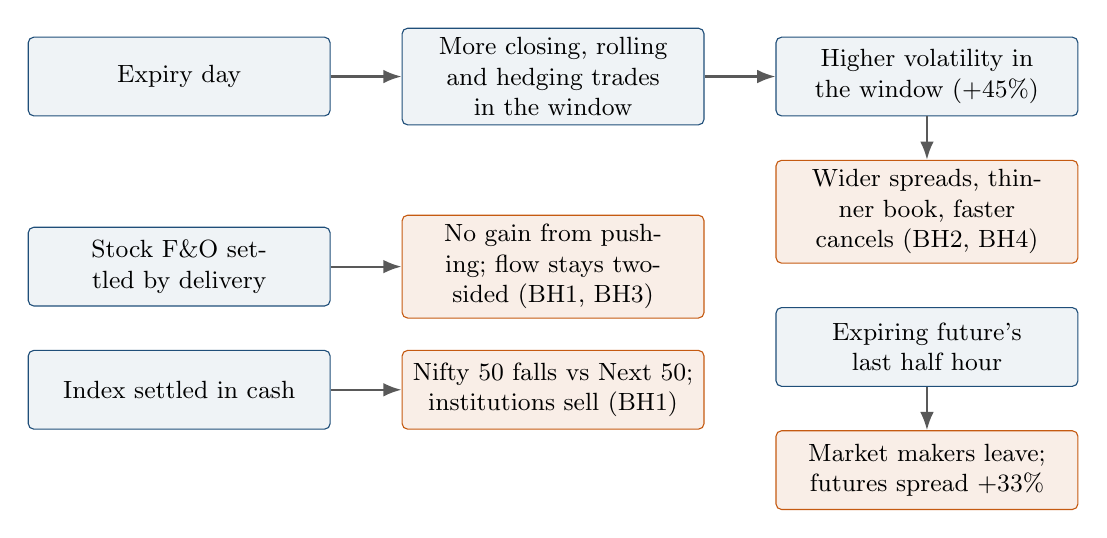
\begin{tikzpicture}[font=\small, node distance=0.55cm and 0.9cm,
  box/.style={draw=iimblue,fill=iimblue!7,rounded corners=2pt,align=center,text width=3.6cm,
    minimum height=1cm},
  res/.style={draw=iimorange,fill=iimorange!10,rounded corners=2pt,align=center,text width=3.6cm,
    minimum height=1cm},
  arr/.style={-{Latex},thick,gray!70!black}]
  \node[box] (exp) {Expiry day};
  \node[box,right=of exp] (more) {More closing, rolling and hedging trades in the window};
  \node[box,right=of more] (vol) {Higher volatility in the window (+45\%)};
  \node[res,below=of vol] (cost) {Wider spreads, thinner book, faster cancels (BH2, BH4)};
  \node[box,below=1.4cm of exp] (deliv) {Stock F\&O settled by delivery};
  \node[res,right=of deliv] (nopush) {No gain from pushing; flow stays two-sided (BH1, BH3)};
  \node[box,below=of deliv] (cash) {Index settled in cash};
  \node[res,right=of cash] (index) {Nifty 50 falls vs Next 50; institutions sell (BH1)};
  \node[box,below=of cost] (last) {Expiring future's last half hour};
  \node[res,below=of last] (fut) {Market makers leave; futures spread +33\%};
  \draw[arr] (exp) -- (more); \draw[arr] (more) -- (vol); \draw[arr] (vol) -- (cost);
  \draw[arr] (deliv) -- (nopush); \draw[arr] (cash) -- (index); \draw[arr] (last) -- (fut);
\end{tikzpicture}
\caption{Our explanation of the results in one picture.}
\label{fig:story}
\end{figure}

\begin{center}
\small
\begin{tabularx}{\textwidth}{XX}
\toprule
What we have tested & What we think explains it (not yet proven) \\
\midrule
Stock settlement prices are not pushed & Options open interest per stock is too small to be worth
  pushing \\
Futures are priced off the cash price (delivery) & Window volatility comes partly from option
  (gamma) hedging \\
Nifty 50 falls 6.2 bps vs Next 50 on index expiries & The index fall is institutions closing
  hedges at the settlement price \\
Window costs more, only in F\&O stocks & The 3\% of widening left over is market makers busy in
  options \\
Volatility explains most of the spread, depth and cancel changes & OIB persistence is
  institutions slicing orders \\
No one-sided OIB, in cash or futures & The leftover overnight reversal is a reward for absorbing
  closing orders \\
Next-morning fall is mostly news & The futures widening is market makers avoiding delivery \\
Expiring future's spread +33\% in the window & \\
\bottomrule
\end{tabularx}
\end{center}

Coming back to the question in our title: on expiry day the last half hour of trading in F\&O
stocks gets busier, more volatile and more expensive, but there is no sign that stock settlement
prices are being punched. The structure of the contracts explains a lot of this. Physical delivery
takes away the reason to push a stock's settlement price, and the one settlement that does move
is the Nifty, which is paid out in cash.

% ---------------------------------------------------------------- limits
\section{Limitations and next steps}

\begin{itemize}
  \item \textbf{Only 12 monthly expiries a year.} A few days can drive a result, which is why we
  used randomization tests and looked at each expiry separately.
  \item \textbf{No trader-level positions.} The data identify participant categories, not
  individual traders or their open positions. That is why we cannot prove the hedge-unwinding
  story or rule out a strategy spread across several participants.
  \item \textbf{News is measured indirectly}, through volume and price gaps. A dataset of company
  announcements would let us test the news explanation directly.
  \item \textbf{The index closing value is approximated} by its average over the window (it was
  within a few index points of the published close where we checked).
  \item \textbf{One year (2022).} Weekly stock-index expiries and the rules have changed since.
\end{itemize}

Next steps before the final submission: discuss the hedge-unwinding mechanism with Shubhankar as
suggested; look at participant flows in Nifty 50 stocks on weekly expiries separately; and, if
possible, add company announcement data for the news test.

% ---------------------------------------------------------------- appendix
\appendix
\section{All measures by hypothesis}

Every measure we tested, with the paired test of expiry day against the day before (one pair per
stock and month). P marks the primary measure of each hypothesis.

\begin{center}
\footnotesize
\begin{tabularx}{\textwidth}{lXrrr}
\toprule
ID & Measure & $t$ & $p$ & $d$ \\
\midrule
\multicolumn{5}{l}{\textit{BH1: The settlement price}} \\
1.1 P & Settlement VWAP further from the window's opening mid & 1.26 & 0.209 & 0.030 \\
1.2 & Volume less evenly spread across the window & $-6.48$ & $<0.001$ & $-0.153$ \\
1.3 & $|$Move from 15:00 to 15:30$|$ is larger & 1.80 & 0.072 & 0.042 \\
1.4 & Settlement VWAP further from the closing price & 4.17 & $<0.001$ & 0.098 \\
1.5 & Final minute's VWAP diverges further from the window's & 3.02 & 0.003 & 0.071 \\
1.6 & Less volume at the running VWAP & $-2.74$ & 0.006 & $-0.064$ \\
1.7 & Volume concentrates in the final minute & $-1.71$ & 0.087 & $-0.040$ \\
\multicolumn{5}{l}{\textit{BH2: The cost of trading}} \\
2.1 P & Quoted spread widens & 6.67 & $<0.001$ & 0.158 \\
2.2 & Order book depth falls & $-2.35$ & 0.019 & $-0.055$ \\
2.3 & Price impact per trade is higher & $-0.24$ & 0.814 & $-0.006$ \\
2.4 & Realised variance per minute is higher & 4.90 & $<0.001$ & 0.115 \\
2.5 & Amihud illiquidity is higher & 2.57 & 0.010 & 0.061 \\
2.6 & Spread recovers more slowly after shocks & $-1.52$ & 0.130 & $-0.036$ \\
2.7 & A fixed order moves the price further & 2.46 & 0.014 & 0.058 \\
2.8 & Displayed value in the book falls & $-4.65$ & $<0.001$ & $-0.110$ \\
2.9 & Flow of a given size moves the price further & 7.36 & $<0.001$ & 0.174 \\
\multicolumn{5}{l}{\textit{BH3: One-sided trading}} \\
3.1 P & $|$Order imbalance$|$ over the window is larger & 0.62 & 0.538 & 0.015 \\
3.2 & Depth falls more on one side & $-1.49$ & 0.136 & $-0.035$ \\
3.3 & Submitted orders are more one-sided & 4.19 & $<0.001$ & 0.099 \\
3.4 & Book pressure is more persistent & $-2.78$ & 0.005 & $-0.066$ \\
3.5 & Prices trend rather than oscillate (variance ratio) & $-0.91$ & 0.361 & $-0.022$ \\
3.6 & Signed order flow is more persistent & $-0.81$ & 0.418 & $-0.019$ \\
3.7 & Larger share of price impact is permanent & $-0.81$ & 0.416 & $-0.019$ \\
\multicolumn{5}{l}{\textit{BH4: Order behaviour and participation}} \\
4.1 P & More orders cancelled within one second & 5.63 & $<0.001$ & 0.133 \\
4.2 & Cancellations per entry rise & $-0.42$ & 0.675 & $-0.010$ \\
4.3 & Cancellation counts rise & 12.21 & $<0.001$ & 0.288 \\
4.4 & More resting size is hidden & 0.50 & 0.614 & 0.012 \\
4.5 & Hidden orders larger relative to displayed part & 1.88 & 0.061 & 0.044 \\
4.6 & Hidden size refilled more per unit traded & $-1.89$ & 0.059 & $-0.044$ \\
4.7 & More submitted volume is hidden & 0.25 & 0.805 & 0.006 \\
4.8 & More orders carry a disclosed quantity & 2.96 & 0.003 & 0.070 \\
4.9 & Proprietary volume in the window rises & 3.37 & $<0.001$ & 0.080 \\
4.10 & Algorithmic volume in the window rises & 0.57 & 0.566 & 0.014 \\
4.11 & IOC submission speeds up in the final five minutes & 1.87 & 0.061 & 0.044 \\
4.12 & Algorithmic orders use IOC more often & 0.15 & 0.880 & 0.004 \\
\bottomrule
\end{tabularx}
\end{center}

\section{Code and data}

All our code is on GitHub at
\href{https://github.com/arnav127/nse-fut-analysis}{\texttt{github.com/arnav127/nse-fut-analysis}}.
The repository's README explains how to run it. The table below links each part of this report
to the code that produces it.

\begin{center}
\footnotesize
\begin{tabularx}{\textwidth}{>{\raggedright\arraybackslash}p{5.2cm}X}
\toprule
Part of the report & Code \\
\midrule
Decoding the raw NSE files & \href{https://github.com/arnav127/nse-fut-analysis/tree/main/stage1_parse}{\texttt{stage1\_parse/}} and our parser
  \href{https://github.com/arnav127/nsetick}{\texttt{nsetick}} \\
Choosing the three groups of stocks & \href{https://github.com/arnav127/nse-fut-analysis/blob/main/scripts/build_universe.py}{\texttt{scripts/build\_universe.py}} \\
Placebo check (Nifty 500, turnover rank) & \href{https://github.com/arnav127/nse-fut-analysis/blob/main/stage9_tape/placebo_check.py}{\texttt{stage9\_tape/placebo\_check.py}} \\
Rebuilding the order book & \href{https://github.com/arnav127/nse-fut-analysis/tree/main/stage4_clob}{\texttt{stage4\_clob/}} \\
Order book measures in the window & \href{https://github.com/arnav127/nse-fut-analysis/tree/main/stage6_insights}{\texttt{stage6\_insights/}} \\
The four hypotheses and paired tests & \href{https://github.com/arnav127/nse-fut-analysis/blob/main/stage8_report/stat_tests.py}{\texttt{stage8\_report/stat\_tests.py}} \\
Full-year data, reversal, order imbalance, flows & \href{https://github.com/arnav127/nse-fut-analysis/blob/main/stage9_tape/settlement_tests.py}{\texttt{stage9\_tape/settlement\_tests.py}} \\
Next-morning fall and news & \href{https://github.com/arnav127/nse-fut-analysis/blob/main/stage9_tape/overnight_tests.py}{\texttt{stage9\_tape/overnight\_tests.py}} \\
Nifty 50 vs Nifty Next 50 & \href{https://github.com/arnav127/nse-fut-analysis/blob/main/stage9_tape/index_tests.py}{\texttt{stage9\_tape/index\_tests.py}} \\
Hedge unwinding and open interest & \href{https://github.com/arnav127/nse-fut-analysis/blob/main/stage9_tape/hedge_tests.py}{\texttt{stage9\_tape/hedge\_tests.py}},
  \href{https://github.com/arnav127/nse-fut-analysis/blob/main/stage9_tape/index_deriv_trades.py}{\texttt{index\_deriv\_trades.py}} \\
Spread, depth and volatility (BH2, BH4) & \href{https://github.com/arnav127/nse-fut-analysis/blob/main/stage9_tape/followups.py}{\texttt{stage9\_tape/followups.py}},
  \href{https://github.com/arnav127/nse-fut-analysis/blob/main/stage9_tape/book_profile.py}{\texttt{book\_profile.py}} \\
BH2 panel regression & \href{https://github.com/arnav127/nse-fut-analysis/blob/main/stage9_tape/bh2_panel.py}{\texttt{stage9\_tape/bh2\_panel.py}} \\
Futures pricing and strike pinning & \href{https://github.com/arnav127/nse-fut-analysis/blob/main/stage6_insights/s7_futures_convergence.py}{\texttt{s7\_futures\_convergence.py}},
  \href{https://github.com/arnav127/nse-fut-analysis/blob/main/stage6_insights/s8_strike_pinning.py}{\texttt{s8\_strike\_pinning.py}} \\
Futures trades and order books & \href{https://github.com/arnav127/nse-fut-analysis/blob/main/stage9_tape/futures_tape.py}{\texttt{stage9\_tape/futures\_tape.py}},
  \href{https://github.com/arnav127/nse-fut-analysis/blob/main/stage9_tape/futures_book.py}{\texttt{futures\_book.py}} \\
Charts in this report & \href{https://github.com/arnav127/nse-fut-analysis/blob/main/report/make_figures.py}{\texttt{report/make\_figures.py}} \\
\bottomrule
\end{tabularx}
\end{center}

\paragraph{Data.} The NSE's historical order, trade and index files are licensed, so they are not
in the repository. The public data we used can be downloaded from the NSE:
\begin{itemize}
  \item Daily F\&O bhavcopy (open interest by contract):
  \href{https://archives.nseindia.com/content/historical/DERIVATIVES/}{NSE derivatives archive}
  \item Participant-wise open interest:
  \href{https://archives.nseindia.com/content/nsccl/}{NSE clearing archive}
  (one file per day,\\ \texttt{fao\_participant\_oi\_DDMMYYYY.csv})
  \item Nifty 50 and Nifty 500 constituents: NSE's index constituent files
  (\href{https://www.niftyindices.com}{\texttt{niftyindices.com}}), archived copies from 2022.
\end{itemize}

\end{document}
